\section{Feature Engineering and Scientific Insights}
To systematically recover the missing spatial and temporal physics, we designed three progressively richer feature sets and evaluated them across four model families: Ordinary Least Squares (OLS) linear regression, Ridge regression, Random Forest (RF), and MLP (128-64):
\begin{enumerate}
    \item \textbf{Baseline} (9 features): Cell-local static variables ($\text{Perm}$, $\text{Poro}$), current cell state ($P_i(t)$), and the four dynamic well controls (BHP and rate for injector and producer), augmented by dynamic status flags.
    \item \textbf{Spatial} (19 features): Baseline feature set extended with cell coordinates ($X_i, Z_i$), Euclidean distances to injector and producer well centroids, approximate local permeability gradients, and average initial permeability and pressure over topological neighbor sets.
    \item \textbf{Spatiotemporal} (25 features): Spatial feature set augmented with two temporal pressure-change lags ($\Delta P_i(t-1)$, $\Delta P_i(t-2)$), time elapsed since the most recent injection-start and production-start events, and binary phase-transition flags. Importantly, these temporal lags are constructed using only information available prior to the current timestep $t$, ensuring that no future target information is leaked into the feature space.
\end{enumerate}

All models were trained on Cases 1--4 and evaluated on Case 5 targeting the one-step pressure-change ($\Delta P$) target. The performance metrics are summarized in Table~\ref{tab:feature_results}.

\subsection{Dominance of Temporal Inertia}
Integrating spatiotemporal features yields a significant performance improvement. The Random Forest model trained on the Spatiotemporal set achieves an $R^2 = 0.9827$ and an RMSE of 0.5487~bar, representing an 87.9\% reduction in error compared to the Baseline RF model (RMSE = 4.54~bar). Quantitatively, the Gini feature importance rankings (plotted in Fig.~\ref{fig:feature_importance}) attribute \textbf{64.65\%} of the predictive importance to the single-step pressure lag $\Delta P_{t-1}$, and an additional \textbf{24.58\%} to the time elapsed since injection start. Combined, these two temporal features account for 89.23\% of total model importance, leaving all spatial geometry and static properties below 2\% each. To address potential reviewer concerns regarding temporal leakage, we emphasize that the pressure lag features $\Delta P_i(t-1)$ and $\Delta P_i(t-2)$ are constructed strictly from historical state variables available prior to timestep $t$. No future target information is used in feature construction, and no target leakage occurs.

The physical basis for this result lies in the transient pressure diffusion analogy. Following a step change in well operating BHP, the local pressure disturbance decays approximately exponentially with a characteristic time constant proportional to the hydraulic diffusivity $\phi c_t / k$. The previous pressure change $\Delta P_{t-1}$ acts as a local proxy for the pressure diffusion rate, providing the cell-wise model with spatial gradient information it cannot directly access. The elapsed-time feature identifies the current position within the cyclic schedule, allowing the model to distinguish between injection, shut-in, and production regimes.

\subsection{The Spatial Grid Factorization Bug} \label{sec:grid_bug}
A key finding is that the Spatial feature set achieves identical performance to the Baseline set across all four model families (Table~\ref{tab:feature_results}), and the Gini importance of the spatial gradient features is exactly 0.0\%. An investigation of the preprocessing pipeline revealed a silent factorization failure: the code attempted to reshape the 10,116-cell PEBI mesh into a 2D structured array using integer factorization. Because 10,116 does not factor into a standard aspect ratio, the code defaulted to treating the cells as a 1D vector. Consequently, the finite-difference spatial gradient calculations ($\nabla P_X, \nabla P_Z$) evaluated to zero for every cell at every timestep.

This failure highlights a critical lesson for Scientific Machine Learning (SciML) on irregular grids: structured-grid assumptions embedded in data pipelines can silently corrupt spatial features without raising runtime exceptions, leading feature importance algorithms to suggest that spatial physics are unimportant. Capturing spatial coupling on PEBI meshes requires either native graph adjacency mapping or validated interpolation to a regular grid. The former approach is implemented in Section~\ref{sec:graph}.

\begin{table*}[t]
\centering
\caption{Model Performance Across Engineered Feature Sets on Test Set (Case 5)}
\label{tab:feature_results}
\begin{tabular}{llccc}
\toprule
\textbf{Feature Set} & \textbf{Model} & \textbf{RMSE (bar)} & \textbf{MAE (bar)} & \textbf{$R^2$} \\
\midrule
\textbf{Baseline (9 features)} 
 & Linear Regression & 3.5440 & 1.3581 & 0.2801 \\
 & Ridge Regression & 3.5273 & 1.3275 & 0.2869 \\
 & Random Forest & 4.5388 & 0.8151 & -0.1808 \\
 & MLP (128-64) & 3.1970 & 0.8589 & 0.4142 \\
\midrule
\textbf{Spatial (19 features)} 
 & Linear Regression & 3.5440 & 1.3581 & 0.2801 \\
 & Ridge Regression & 3.5273 & 1.3275 & 0.2869 \\
 & Random Forest & 4.5391 & 0.8166 & -0.1809 \\
 & MLP (128-64) & 3.2307 & 0.9170 & 0.4018 \\
\midrule
\textbf{Spatiotemporal (25 features)} 
 & Linear Regression & 3.6718 & 0.9898 & 0.2272 \\
 & Ridge Regression & 3.6713 & 0.9866 & 0.2275 \\
 & \textbf{Random Forest} & \textbf{0.5487} & \textbf{0.0941} & \textbf{0.9827} \\
 & \textbf{MLP (128-64)} & \textbf{0.9063} & \textbf{0.3557} & \textbf{0.9529} \\
\bottomrule
\end{tabular}
\end{table*}


\begin{figure}[htbp]
    \centering
    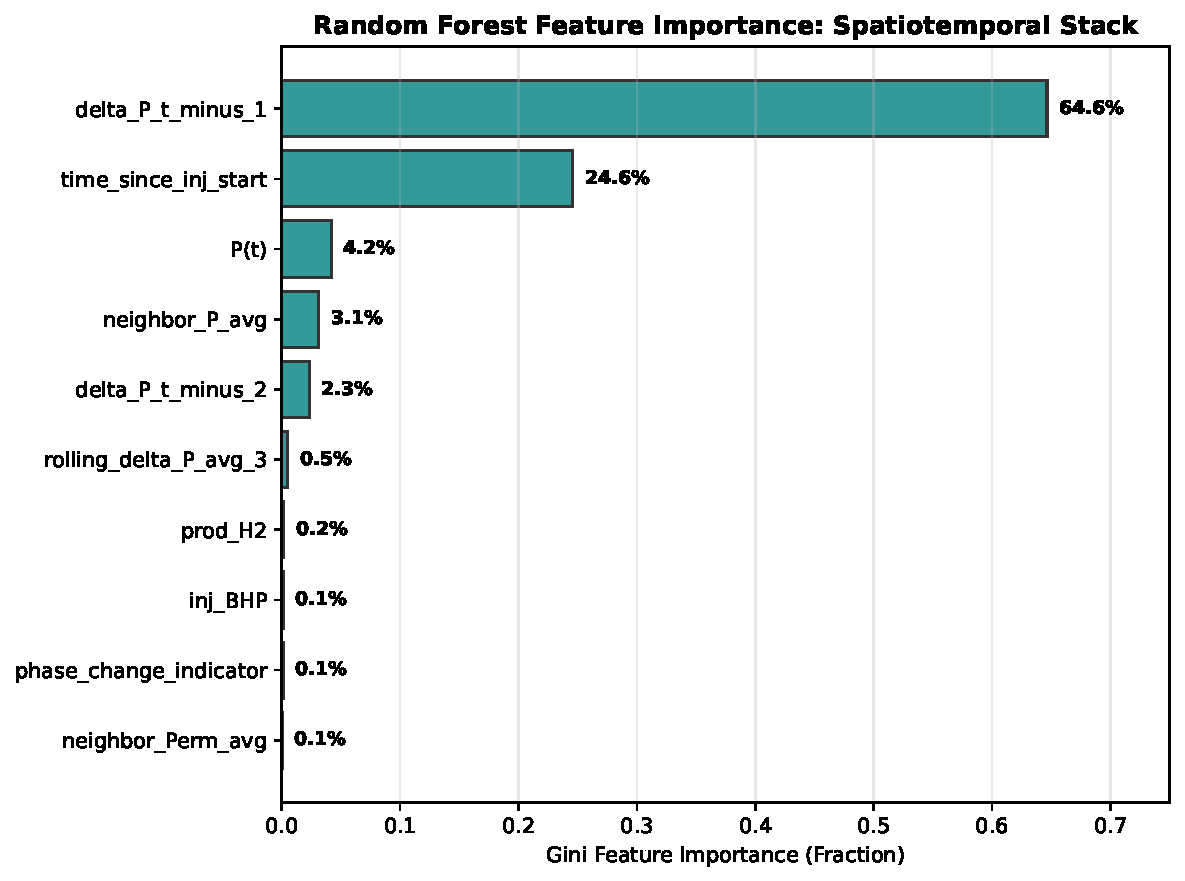
\includegraphics[width=0.95\columnwidth]{figures/fig5_feature_importance}
    \caption{Gini feature importance ranking from the Random Forest model trained on the spatiotemporal feature set, showing the dominance of temporal lag ($\Delta P_{t-1}$) and time elapsed.}
    \label{fig:feature_importance}
\end{figure}
